\section{Estimation for QCD multijet events \label{sec:qcd}}

One of the major challenges for searches of new physics in the jets + \met final state is the control of background events from QCD multijet
production. The difficulties in the determination of precise estimates for this background stem from the large cross sections expected in the
high-energy, high-luminosity hadron collider environment at the LHC, which are further compounded by the lack of precise theoretical
predictions for the cross sections and kinematic properties of multijet events. Hence, without special consideration and treatment,
significant uncertainties on large background expectations can overwhelm any potential sensitivity to new physics signatures.


Because of the analsyis appraoch to suppress the QCD multijet background to a
negligible level -   sub-percent level -  we prefer a conservative uncertainty on a negligible contribution is
 over a procedure that attempts to accurately estimate a
non-negligible contribution from multijet events. 


Any contamination from QCD multijet events is controlled primarily through the \alphat and \bdphi variables. The \alphat variable is able
to distiguish with high efficiency the sources of ``fake'' \met, such as jet energy mismeasurement, from those with ``genuine'' \met, such
as neutrinos. The \bdphi variable is also very efficient at identifying jets that suffer under-measurements, as well as
over-measurements, in (otherwise balanced) multijet events. The variable is also particularly suited to identifying multijet events
that exhibit significant \met due to the production of neutrinos (collinear with a jet axis) in semileptonic heavy-flavour decays. Both
variables are individually capable of reducing the yields from multijet events by several orders of magnitude, and combined provide
an extremely robust method to reject multijet events. 

We determing the ratio \rmhtmet per (\njet,\scalht) bin from simulation. The ratio is determined by applying the (\scalht-dependent)
\alphat and \bdphi requirements. For the region $\scalht > 800\gev$, the requirement $\mht > 130\gev$ is made instead of \alphat. 
No \alphat nor \mht requirements are imposed for events in the monojet category.

Each ratio \rmhtmet is then used as a multiplier on data counts per (\njet,\scalht) bin obtained in the
\mhtmet data sideband. Expected background from $V$+jets and \ttbar are then subtracted to obtain the expected number of 
QCD multijet background events ($\mathcal{Q}$) for each bin of the QCD enriched signal region.

The product $\mathcal{Q} \times \mhtmet$ then provides an estimate of the level of QCD multijet events in
each (\njet,\scalht) bin of the signal region. The estimation is inclusive in \nb\ and \mht for each
(\njet,\scalht) bin. 


The number multijet events passing/failing the $\mhtmet < 1.25$ requirement is then determined for simuations for each
of these bins.

Figure~\ref{fig:qcd_pred} shows the expected number of QCD multijet
 in the signal region bins for each bin in \njet and \scalht and also
th relative contributions of QCD multijet over the EWK backgrounds. One sees that the
fraction of QCD events is indeed negligible.




\begin{figure}[!h]
  \centering
  \subfigure[QCD multijet predictions in the signal region.\label{fig:qcd_pred}]{
    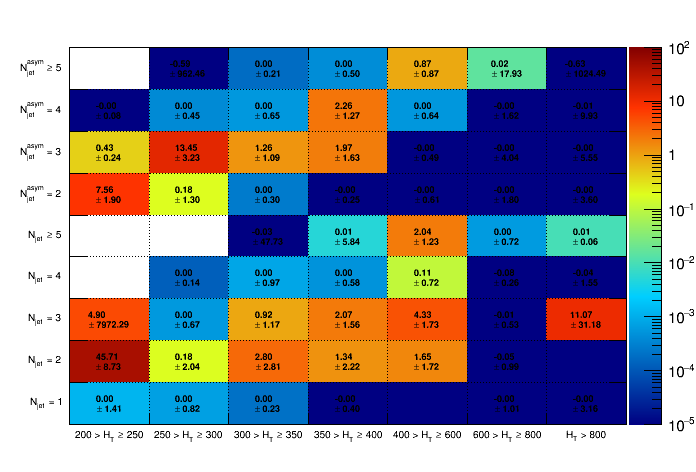
\includegraphics[width=0.5\textwidth]{figures/qcd/v2/DataNoEwk_SigTrig_QCDPred_NJet_vs_HT_bDPhigt0p5_Log}
  } 
  \subfigure[Ratio of predicted multijet and non-multijet yields.\label{fig:qcd_ewk_ratio}]{
    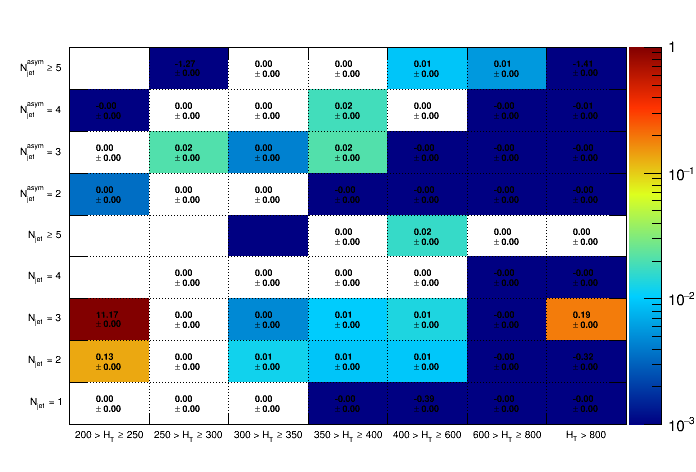
\includegraphics[width=0.5\textwidth]{figures/qcd/v2/DataNoEwk_SigTrig_QCDPredDivEwk_NJet_vs_HT_bDPhigt0p5_Log}
  } \\
  \caption{a) Expected number of QCD multijet events determined from
    simulation, binned according to \njet and \scalht in the signal region and b) the ratio to remaining EWK background }
  \label{fig:qcd_plots}
\end{figure}
